\documentclass[a4paper, 11pt]{article}
\usepackage{graphicx}
\usepackage{multicol}
\usepackage{tabularx}
\usepackage{enumitem}
\usepackage[a4paper, margin=1.8cm]{geometry}
\usepackage{listings}
\usepackage{amssymb}
\usepackage{gvv}
\usepackage{gvv-book}
\usepackage{amsmath}
\usepackage{setspace}
\usepackage{caption}
\usepackage{tfrupee}


\graphicspath{ {./} }

\begin{document}
\begin{center}
    \huge{CS: COMPUTER SCIENCE AND INFORMATION TECHNOLOGY-2021}\\
    \large{EE25BTECH11041 - Naman Kumar}
\end{center}

\begin{enumerate}
    \item The ratio of boys to girls in a class is $7$ to $3$.
    Among the options below, an acceptable value for the total number of students in the class is:
    \begin{enumerate}
        \begin{multicols}{4}
            \item $21$
            \item $37$
            \item $50$
            \item $73$
        \end{multicols}
    \end{enumerate}
    \hfill{\brak{\text{GATE CS 2021}}}

    \item A polygon is convex if, for every pair of points, P and Q belonging to the polygon, the line segment PQ lies completely inside or on the polygon.
    Which one of the following is NOT a convex polygon?
    \begin{enumerate}
        \item 
        \begin{figure}[H]
            \centering
            
\includegraphics[width=0.1\columnwidth]{figs/q2A.png}
            \label{fig:q2}
        \end{figure}
        \item \begin{figure}[H]
            \centering
            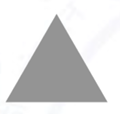
\includegraphics[width=0.1\columnwidth]{figs/q2B.png}
            \label{fig:placeholder}
        \end{figure}
        \item \begin{figure}[H]
            \centering
            
\includegraphics[width=0.1\columnwidth]{figs/q2C.png}
            \label{fig:placeholder}
        \end{figure}
        \item \begin{figure}[H]
            \centering
            
\includegraphics[width=0.1\columnwidth]{figs/q2D.png}
            \label{fig:placeholder}
        \end{figure}
    \end{enumerate}
    \hfill{\brak{\text{GATE CS 2021}}}

    \item Consider the following sentences:
    \begin{enumerate}[label=(\roman*)]
    \centering
        \item Everybody in the class is prepared for the exam.
        \item Babu invited Danish to his home because he enjoys playing chess.
    \end{enumerate}
    Which of the following is the CORRECT observation about the above two sentences?
    \begin{enumerate}
        \item \brak{\text{i}} is grammatically correct and \brak{\text{ii}} is unambiguous
        \item \brak{\text{i}} is grammatically incorrect and \brak{\text{ii}} is unambiguous
        \item \brak{\text{i}} is grammatically correct and \brak{\text{ii}} is ambiguous
        \item \brak{\text{i}} is grammatically incorrect and \brak{\text{ii}} is ambiguous
    \end{enumerate}
    \hfill{\brak{\text{GATE CS 2021}}}

    \item 
    \begin{figure}[h]
        \centering
        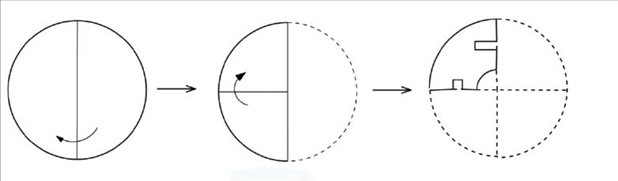
\includegraphics[width=0.8\columnwidth]{figs/q4.png}
        \label{fig:q4}
    \end{figure}
    
    A circular sheet of paper is folded along the lines in the directions shown. The paper, after being punched in the final folded state as shown and unfolded in the reverse order of folding, will look like \underline{\hspace{2cm}}.
    \begin{enumerate}
        \item 
        \begin{figure}[H]
            \centering
            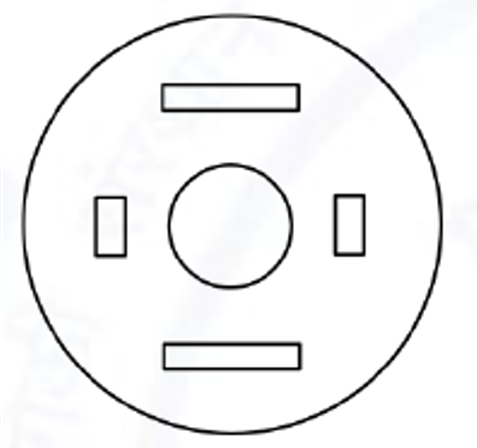
\includegraphics[width=0.1\columnwidth]{figs/q4A.png}
            \label{fig:placeholder}
        \end{figure}
        \item
        \begin{figure}[H]
            \centering
            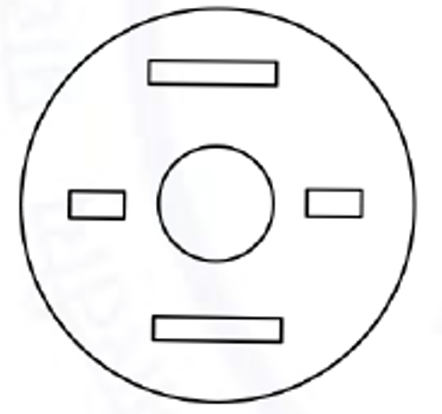
\includegraphics[width=0.1\columnwidth]{figs/q4B.png}
            \label{fig:placeholder}
        \end{figure}
        \item
        \begin{figure}[H]
            \centering
            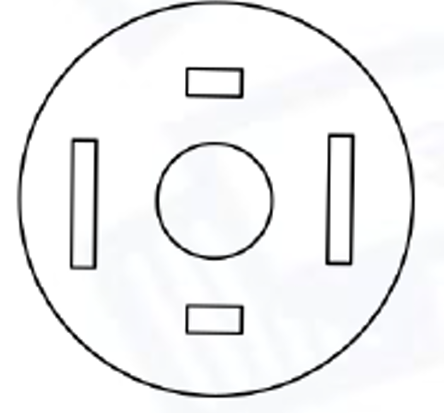
\includegraphics[width=0.1\columnwidth]{figs/q4C.png}
            \label{fig:placeholder}
        \end{figure}
        \item
        \begin{figure}[H]
            \centering
            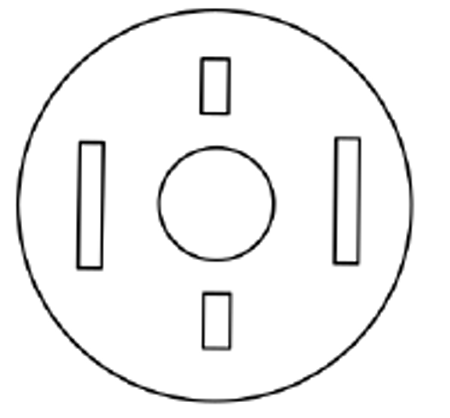
\includegraphics[width=0.1\columnwidth]{figs/q4D.png}
            \label{fig:placeholder}
        \end{figure}
    \end{enumerate}
    \hfill{\brak{\text{GATE CS 2021}}}

    \item \underline{\hspace{2cm}} is to surgery as writer is to \underline{\hspace{2cm}}.\\Which one of the following options maintains a similar logical relation in the above sentence?
    \begin{enumerate}
    \begin{multicols}{2}
        \item Plan, outline
        \item Hospital, library
        \item Doctor, book
        \item Medicine, grammar
    \end{multicols}
    \end{enumerate}
    \hfill{\brak{\text{GATE CS 2021}}}

    \item We have $2$ rectangular sheets of paper, M and N, of dimensions $6$ cm x $1$ cm each. Sheet M is rolled to form an open cylinder by bringing the short edges of the sheet together. Sheet N is cut into equal square patches and assembled to form the largest possible closed cube. Assuming the ends of the cylinder are closed, the ratio of the volume of the cylinder to that of the cube is \underline{\hspace{2cm}}.
    \begin{enumerate}
        \begin{multicols}{2}
            \item $\frac{\pi}{2}$
            \item $\frac{3}{\pi}$
            \item $\frac{9}{\pi}$
            \item $3\pi$
        \end{multicols}
    \end{enumerate}
    \hfill{\brak{\text{GATE CS 2021}}}

    \item 
    \begin{table}[H]
        \centering
        \begin{tabular}{|c|c|c|c|}
            \hline
            \textbf{Items} & \textbf{Cost (\rupee)} & \textbf{Profit \%} & Market Price (\rupee) \\
            \hline
            P & $5,400$ & \dots & 5,860 \\
            Q & \dots & $25$ & 10,000\\
            \hline
        \end{tabular}
        \caption*{}
        \label{tab:q7}
    \end{table}
    Details of prices of two items P and Q are presented in the above table. The ratio of cost of item P to cost of item Q is $3:4$. Discount is calculated as the difference between the marked price and the selling price. The profit percentage is calculated as the ratio of the difference between selling price and cost, to the cost \brak{\text{Profit\%} = \frac{\text{Selling Price} - \text{Cost}}{\text{Cost}} \times 100}.\\The discount on item Q, as a percentage of its marked price, is \underline{\hspace{2cm}}.
    \begin{enumerate}
        \begin{multicols}{4}
            \item $25$
            \item $12.5$
            \item $10$
            \item $5$
        \end{multicols}
    \end{enumerate}
    \hfill{\brak{\text{GATE CS 2021}}}

    \item There are five bags each containing identical sets of ten distinct chocolates. One chocolate is picked from each bag.
    The probability that at least two chocolates are identical is \underline{\hspace{2cm}}.
    \begin{enumerate}
        \item $0.3024$
        \item $0.4235$
        \item $0.6976$
        \item $0.8125$
    \end{enumerate}
    \hfill{\brak{\text{GATE CS 2021}}}

    \item Given below are two statements 1 and 2, and two conclusions I and II.
    
    \textbf{Statement 1:} All bacteria are microorganisms.
    
    \textbf{Statement 2:} All pathogens are microorganisms.
    
    \textbf{Conclusion I:} Some pathogens are bacteria.
    
    \textbf{Conclusion II:} All pathogens are not bacteria.
    Based on the above statements and conclusions, which one of the following options is logically CORRECT?
    \begin{enumerate}
        \item Only conclusion I is correct
        \item Only conclusion II is correct
        \item Either conclusion I or II is correct.
        \item Neither conclusion I nor II is correct.
    \end{enumerate}
    \hfill{\brak{\text{GATE CS 2021}}}

    \item Some people suggest anti-obesity measures \brak{\text{AOM}} such as displaying calorie information in restaurant menus. Such measures sidestep addressing the core problems that cause obesity: poverty and income inequality.\\Which one of the following statements summarizes the passage?
    \begin{enumerate}
        \item The proposed AOM addresses the core problems that cause obesity.
        \item If obesity reduces, poverty will naturally reduce, since obesity causes poverty.
        \item AOM are addressing the core problems and are likely to succeed.
        \item AOM are addressing the problem superficially.
    \end{enumerate}
    \hfill{\brak{\text{GATE CS 2021}}}
    
    \item Suppose that $L_1$ is a regular language and $L_2$ is a context-free language. Which one of the following languages is NOT necessarily context-free?
    \begin{enumerate}
        \begin{multicols}{2}
            \item $L_1 \cap L_2$
            \item $L_1 \cdot L_2$
            \item $L_1 - L_2$
            \item $L_1 \cup L_2$
        \end{multicols}
    \end{enumerate}
    \hfill{\brak{\text{GATE CS 2021}}}
    
    \item Let P be an array containing n integers. Let t be the lowest upper bound on the number of comparisons of the array elements, required to find the minimum and maximum values in an arbitrary array of n elements. Which one of the following choices is correct?
    \begin{enumerate}
        \item $t > 2n-2$
        \item $t > 3 \lceil \frac{n}{2} \rceil$ and $t \le 2n-2$
        \item $t > n$ and $t \le 3 \lceil \frac{n}{2} \rceil$
        \item $t > \lceil \log_2\brak{n} \rceil$ and $t \le n$
    \end{enumerate}
    \hfill{\brak{\text{GATE CS 2021}}}
    
    \item Consider the following three functions.
    \[ f_1 = 10^n \quad f_2 = n^{\log n} \quad f_3 = n^{\sqrt{n}} \]
    Which one of the following options arranges the functions in the increasing order of asymptotic growth rate?
    \begin{enumerate}
        \item $f_3, f_2, f_1$
        \item $f_2, f_1, f_3$
        \item $f_1, f_2, f_3$
        \item $f_2, f_3, f_1$
    \end{enumerate}
    \hfill{\brak{\text{GATE CS 2021}}}
    
    \item Consider the following statements.
    \begin{tabular}{cc}
    $S_1$: & The sequence of procedure calls corresponds to a preorder traversal of the activation tree.\\
    $S_2$:& The sequence of procedure returns corresponds to a postorder traversal of the activation tree.
    \end{tabular}
    Which one of the following options is correct?
    \begin{enumerate}
        \item $S_1$ is true and $S_2$ is false
        \item $S_1$ is false and $S_2$ is true
        \item $S_1$ is true and $S_2$ is true
        \item $S_1$ is false and $S_2$ is false
    \end{enumerate}
    \hfill{\brak{\text{GATE CS 2021}}}
    \item Consider the following statements.\\
    \begin{tabular}{cc}
    $S_1$: &  Every SLR\brak{1} grammar is unambiguous but there are certain unambiguous grammars that are not SLR\brak{1}.\\
    $S_2$: &  For any context-free grammar, there is a parser that takes at most $O\brak{n^3}$ time to parse a string of length n.
    \end{tabular}
    Which one of the following options is correct?
    \begin{enumerate}
        \item $S_1$ is true and $S_2$ is false
        \item $S_1$ is false and $S_2$ is true
        \item $S_1$ is true and $S_2$ is true
        \item $S_1$ is false and $S_2$ is false
    \end{enumerate}
    \hfill{\brak{\text{GATE CS 2021}}}
    
    \item Let the representation of a number in base 3 be 210. What is the hexadecimal representation of the number?
    \begin{enumerate}
        \begin{multicols}{4}
            \item 15
            \item 21
            \item D2
            \item 528
        \end{multicols}
    \end{enumerate}
    \hfill{\brak{\text{GATE CS 2021}}}
    
    \item Let p and q be two propositions. Consider the following two formulae in propositional logic.\\
    \begin{tabular}{cc}
    \centering
    $S_1:$&$(\neg p \land (p \lor q)) \rightarrow q$\\
    $S_2:$&$ q \rightarrow (\neg p \land (p \lor q))$
    \end{tabular}\\
    Which one of the following choices is correct?
    \begin{enumerate}
        \item Both $S_1$ and $S_2$ are tautologies.
        \item $S_1$ is a tautology but $S_2$ is not a tautology.
        \item $S_1$ is not a tautology but $S_2$ is a tautology.
        \item Neither $S_1$ nor $S_2$ is a tautology.
    \end{enumerate}
    \hfill{\brak{\text{GATE CS 2021}}}
    
    \item Consider the following two statements.\\
    \begin{tabular}{cc}
        $S_1$: & Destination MAC address of an ARP reply is a broadcast address. \\
        $S_2$: & Destination MAC address of an ARP request is a broadcast address.
    \end{tabular}\\
    Which one of the following choices is correct?
    \begin{enumerate}
        \item Both $S_1$ and $S_2$ are true.
        \item $S_1$ is true and $S_2$ is false.
        \item $S_1$ is false and $S_2$ is true.
        \item Both $S_1$ and $S_2$ are false.
    \end{enumerate}
    \hfill{\brak{\text{GATE CS 2021}}}
    
    \item Consider the following array.
    
    \begin{center}
        23 \quad 32 \quad 45 \quad 69 \quad 72 \quad 73 \quad 89 \quad 97
    \end{center}
    Which algorithm out of the following options uses the least number of comparisons \brak{\text{among the array elements}} to sort the above array in ascending order?
    \begin{enumerate}
        \begin{multicols}{2}
            \item Selection sort
            \item Mergesort
            \item Insertion sort
            \item Quicksort using the last element as pivot
        \end{multicols}
    \end{enumerate}
    \hfill{\brak{\text{GATE CS 2021}}}
    
    \item A binary search tree T contains n distinct elements. What is the time complexity of picking an element in T that is smaller than the maximum element in T?
    \begin{enumerate}
        \begin{multicols}{4}
            \item $\Theta\brak{n \log n}$
            \item $\Theta\brak{n}$
            \item $\Theta\brak{\log n}$
            \item $\Theta\brak{1}$
        \end{multicols}
    \end{enumerate}
    \hfill{\brak{\text{GATE CS 2021}}}

    \item In the context of operating systems, which of the following statements is/are correct with respect to paging?
    \begin{enumerate}
        \item Paging helps solve the issue of external fragmentation.
        \item Page size has no impact on internal fragmentation.
        \item Paging incurs memory overheads.
        \item Multi-level paging is necessary to support pages of different sizes.
    \end{enumerate}
    \hfill{\brak{\text{GATE CS 2021}}}
    
    \item Let $\langle M \rangle$ denote an encoding of an automaton M. Suppose that $\Sigma = \{0,1\}$. Which of the following languages is/are NOT recursive?
    \begin{enumerate}
        \item $L = \{\langle M \rangle | M \text{ is a DFA such that } L\brak{M} = \emptyset\}$
        \item $L = \{\langle M \rangle | M \text{ is a DFA such that } L\brak{M} = \Sigma^*\}$
        \item $L = \{\langle M \rangle | M \text{ is a PDA such that } L\brak{M} = \emptyset\}$
        \item $L = \{\langle M \rangle | M \text{ is a PDA such that } L\brak{M} = \Sigma^*\}$
    \end{enumerate}
    \hfill{\brak{\text{GATE CS 2021}}}
    
    \item Suppose a database system crashes again while recovering from a previous crash. Assume checkpointing is not done by the database either during the transactions or during recovery. Which of the following statements is/are correct?
    \begin{enumerate}
        \item The same undo and redo list will be used while recovering again.
        \item The system cannot recover any further.
        \item All the transactions that are already undone and redone will not be recovered again.
        \item The database will become inconsistent.
    \end{enumerate}
    \hfill{\brak{\text{GATE CS 2021}}}
    
    \item Which of the following standard C library functions will always invoke a system call when executed from a single-threaded process in a UNIX/Linux operating system?
    \begin{enumerate}
    \begin{multicols}{4}
        \item exit
        \item malloc
        \item sleep
        \item strlen
    \end{multicols}
    \end{enumerate}
    \hfill{\brak{\text{GATE CS 2021}}}
    
    \item Consider a linear list based directory implementation in a file system. Each directory is a list of nodes, where each node contains the file name along with the file metadata, such as the list of pointers to the data blocks. Consider a given directory `foo`. Which of the following operations will necessarily require a full scan of `foo` for successful completion?
    \begin{enumerate}
    \begin{multicols}{2}
        \item Creation of a new file in `foo`
        \item Deletion of an existing file from `foo`
        \item Renaming of an existing file in `foo`
        \item Opening of an existing file in `foo`
    \end{multicols}
    \end{enumerate}
    \hfill{\brak{\text{GATE CS 2021}}}
    
    \item In an undirected connected planar graph G, there are eight vertices and five faces. The number of edges in G is \underline{\hspace{2cm}}.
    
    \hfill{\brak{\text{GATE CS 2021}}}
    
    \item Consider the following undirected graph with edge weights as shown:
    \begin{figure}[H]
        \centering
        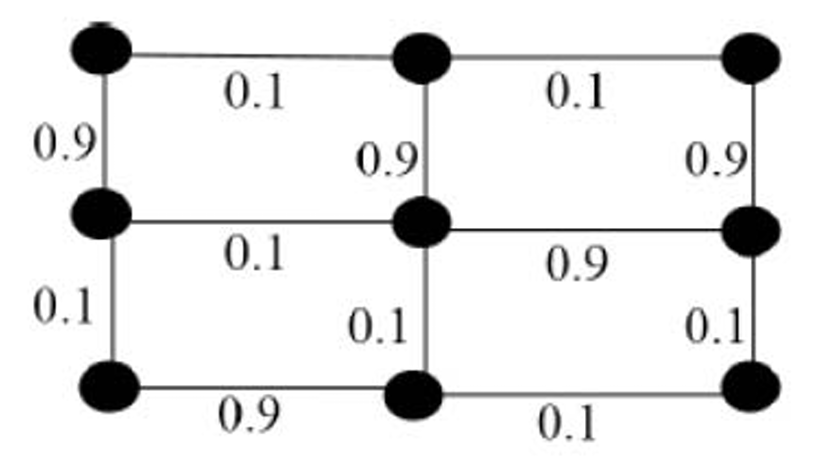
\includegraphics[width=0.5\columnwidth]{figs/q27.png}
        \label{fig:q17}
    \end{figure}
    The number of minimum-weight spanning trees of the graph is \underline{\hspace{2cm}}.
    
    \hfill{\brak{\text{GATE CS 2021}}}
    
    \item The lifetime of a component of a certain type is a random variable whose probability density function is exponentially distributed with parameter 2. For a randomly picked component of this type, the probability that its lifetime exceeds the expected lifetime \brak{\text{rounded to 2 decimal places}} is \underline{\hspace{2cm}}.
    
    \hfill{\brak{\text{GATE CS 2021}}}
    
    \item There are 6 jobs with distinct difficulty levels, and 3 computers with distinct processing speeds. Each job is assigned to a computer such that:
    \begin{itemize}
        \item The fastest computer gets the toughest job and the slowest computer gets the easiest job.
        \item Every computer gets at least one job.
    \end{itemize}
    The number of ways in which this can be done is \underline{\hspace{2cm}}.
    
    \hfill{\brak{\text{GATE CS 2021}}}
    
    \item Consider the following expression.
    \[ \lim_{x\rightarrow-3}\frac{\sqrt{2x+22}-4}{x+3} \]
    The value of the above expression \brak{\text{rounded to 2 decimal places}} is \underline{\hspace{2cm}}.
    
    \hfill{\brak{\text{GATE CS 2021}}}
    
    \item Consider the following sequence of operations on an empty stack.\\
    \begin{center}
    \textit{
    push\brak{54}; push\brak{52}; pop\brak{}; push\brak{55}; push\brak{62}; s=pop\brak{};
    }
    \end{center}
    Consider the following sequence of operations on an empty queue.
    \begin{center}
    \textit{
    enqueue\brak{21}; enqueue\brak{24}; dequeue\brak{}; enqueue\brak{28}; enqueue\brak{32}; q = dequeue\brak{};
    }
    \end{center}
    The value of $s+q$ is \underline{\hspace{2cm}}.
    \hfill{\brak{\text{GATE CS 2021}}}
    
    \item Consider a computer system with a byte-addressable primary memory of size $2^{32}$ bytes. Assume the computer system has a direct-mapped cache of size 32 KB \brak{\text{1 KB = 210 bytes}}, and each cache block is of size 64 bytes. The size of the tag field is \underline{\hspace{2cm}} bits.
    \hfill{\brak{\text{GATE CS 2021}}}
    
    \item A relation $r\brak{A,B}$ in a relational database has 1200 tuples. The attribute A has integer values ranging from 6 to 20, and the attribute B has integer values ranging from 1 to 20. Assume that the attributes A and B are independently distributed.\\The estimated number of tuples in the output of $\sigma_{\brak{A>10} \lor \brak{B=18}}\brak{r}$ is \underline{\hspace{2cm}}.
    \hfill{\brak{\text{GATE CS 2021}}}
    \item Consider the following representation of a number in IEEE 754 single-precision floating point format with a bias of 127.
    \begin{center}   
    S:1 E: 10000001 F: 11110000000000000000000
    \end{center}
    Here S, E and F denote the sign, exponent and fraction components of the floating point representation.\\
    The decimal value corresponding to the above representation \brak{\text{rounded to 2 decimal places}} is \underline{\hspace{2cm}}.
    \hfill{\brak{\text{GATE CS 2021}}}
    
    \item Three processes arrive at time zero with CPU bursts of 16, 20 and 10 milliseconds. If the scheduler has prior knowledge about the length of the CPU bursts, the minimum achievable average waiting time for these three processes in a non-preemptive scheduler \brak{\text{rounded to nearest integer}} is \underline{\hspace{2cm}} milliseconds.
    
    \hfill{\brak{\text{GATE CS 2021}}}
    
    \item Consider the following grammar \brak{\text{that admits a series of declarations, followed by expressions}} and the associated syntax directed translation \brak{\text{SDT}} actions, given as pseudo-code:\\
    \begin{tabular}{ccc}
        P & $\rightarrow$ & $D^* E^*$\\
        D & $\rightarrow$ & $\text{int ID \{record that ID.lexeme is of type int\}}$ \\
        D & $\rightarrow$ & $\text{bool ID \{record that ID.lexeme is of type bool\}}$\\
        E & $\rightarrow$ & $E_1 + E_2 \text{\{check that } E_1\text{.type} = E_2\text{.type} = \text{int; set E.type:= int\}}$\\
        E & $\rightarrow$ & $!E_1 \text{\{check that } E_1\text{.type} = \text{bool; set E.type:= bool\}}$\\
        E & $\rightarrow$ & $ \text{ID \{set E.type:= lookup(ID.lexeme)\}}$\\
    \end{tabular}    
    With respect to the above grammar, which one of the following choices is correct?
    \begin{enumerate}
        \item The actions can be used to correctly type-check any syntactically correct program.
        \item The actions can be used to type-check syntactically correct integer variable declarations and integer expressions.
        \item The actions can be used to type-check syntactically correct boolean variable declarations and boolean expressions.
        \item The actions will lead to an infinite loop.
    \end{enumerate}
    \hfill{\brak{\text{GATE CS 2021}}}
    
    \item The following relation records the age of 500 employees of a company, where empNo \brak{\text{indicating the employee number}} is the key:\\
    \begin{center} 
    empAge\brak{\underline{empNo}, age}
    \end{center}
    Consider the following relational algebra expression:
    \begin{center}
    $\Pi_{\text{empNo}}\brak{\text{empAge} \bowtie_{\brak{\text{age} > \text{age1}}} \rho_{\text{empNo1, age1}}\brak{\text{empAge}}}$
    \end{center}
    What does the above expression generate?
    \begin{enumerate}
        \item Employee numbers of only those employees whose age is the maximum.
        \item Employee numbers of only those employees whose age is more than the age of exactly one other employee.
        \item Employee numbers of all employees whose age is not the minimum.
        \item Employee numbers of all employees whose age is the minimum.
    \end{enumerate}
    \hfill{\brak{\text{GATE CS 2021}}}
    
    \item Consider a 3-bit counter, designed using T flip-flops, as shown below:
    \begin{figure}[h]
        \centering
        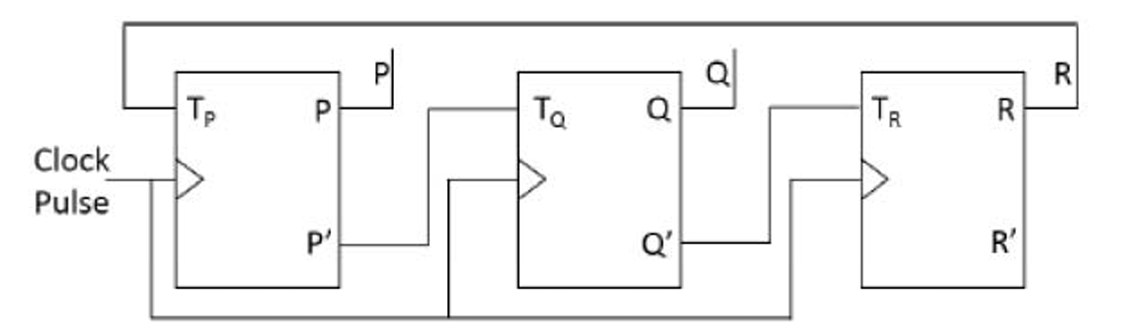
\includegraphics[width=0.6\columnwidth]{figs/q38.png}
        \label{fig:placeholder}
    \end{figure}
    Assuming the initial state of the counter given by PQR as 000, what are the next three states?
    \begin{enumerate}
        \begin{multicols}{2}
            \item 011, 101, 000
            \item 001, 010, 111
            \item 011, 101, 111
            \item 001, 010, 000
        \end{multicols}
    \end{enumerate}
    \hfill{\brak{\text{GATE CS 2021}}}
    
    \item Assume that a 12-bit Hamming codeword consisting of 8-bit data and 4 check bits is $d_8 d_7 d_6 d_5 c_8 d_4 d_3 d_2 c_4 d_1 c_2 c_1$, where the data bits and the check bits are given in the following tables:\\
    \begin{minipage}{0.45\textwidth}
    \centering
        \begin{tabular}{|c|c|c|c|c|c|c|c|}
            \hline
            \multicolumn{8}{|c|}{\textbf{Data bits}} \\
            \hline
            $d_8$ & $d_7$ & $d_6$ & $d_5$ & $d_4$ & $d_3$ & $d_2$ & $d_1$ \\
            \hline
            1 & 1 & 0 & z & 0 & 1 & 0 & 1 \\
            \hline
    \end{tabular}
    \end{minipage}
    \begin{minipage}{0.45\textwidth}
    \centering
        \begin{tabular}{|c|c|c|c|}
            \hline
            \multicolumn{4}{|c|}{\textbf{Check Bits}} \\
            \hline
            $c_8$&$c_4$&$c_2$&$c_1$\\
            \hline
            y & 0 & 1 & 0\\
            \hline
    \end{tabular}
    \end{minipage}
    Which one of the following choices gives the correct values of z and y?
    \begin{enumerate}
        \item z is 0 and y is 0.
        \item z is 0 and y is 1.
        \item z is 1 and y is 0.
        \item z is 1 and y is 1.
    \end{enumerate}
    \hfill{\brak{\text{GATE CS 2021}}}
    
    \item Consider the following recurrence relation.
    \[ T\brak{n} = \begin{cases} T\brak{n/2} + T\brak{2n/5} + 7n & \text{if } n > 0 \\ 1 & \text{if } n=0 \end{cases} \]
    Which one of the following options is correct?
    \begin{enumerate}
        \begin{multicols}{2}
            \item $T\brak{n} = \Theta\brak{n^{5/2}}$
            \item $T\brak{n} = \Theta\brak{n \log n}$
            \item $T\brak{n} = \Theta\brak{n}$
            \item $T\brak{n} = \Theta\brak{\brak{\log n}^{5/2}}$
        \end{multicols}
    \end{enumerate}
    \hfill{\brak{\text{GATE CS 2021}}}
    
    \item Consider the following context-free grammar where the set of terminals is \{a, b c, d. f\}.\\
    $S \rightarrow daT | Rf$
    
    $T \rightarrow aS | baT | \epsilon$
    
    $R \rightarrow caTR | \epsilon$
    
    The following is a partially-filled LL\brak{1} parsing table.
    
    \begin{table}[h]
        \centering
        \begin{tabular}{ccccccc}
            \hline
             & a & b & c & d & f & \$ \\
            \hline
            S & & & \textcircled{1} & $S \rightarrow daT$ & \textcircled{2} & \\
            \hline
            T & $T \rightarrow aS$ & $T \rightarrow baT$ &\textcircled{3} & &$T\rightarrow\epsilon$& \textcircled{4} \\
            \hline
            R & & & $R \rightarrow caTR$ & & $R \rightarrow \epsilon$ & \\
            \hline
        \end{tabular}
        \caption*{}
    \end{table}
    Which one of the following choices represents the correct combination for the numbered cells in the parsing table \brak{\text{"blank" denotes that the corresponding cell is empty}}?
    \begin{enumerate}
        \item \textcircled{1} $S \rightarrow Rf$ \textcircled{2} $S \rightarrow Rf$ \textcircled{3} $T \rightarrow \epsilon$ \textcircled{4} $T \rightarrow \epsilon$
        \item \textcircled{1} blank \textcircled{2} $S \rightarrow Rf$ \textcircled{3} $T \rightarrow \epsilon$ \textcircled{4} $T \rightarrow \epsilon$
        \item \textcircled{1} $S \rightarrow Rf$ \textcircled{2} blank \textcircled{3} blank \textcircled{4} $T \rightarrow \epsilon$
        \item \textcircled{1} blank \textcircled{2} $S \rightarrow Rf$ \textcircled{3} blank \textcircled{4} blank
    \end{enumerate}
    \hfill{\brak{\text{GATE CS 2021}}}
    \item Let $r_i\brak{z}$ and $w_i\brak{z}$ denote read and write operations respectively on a data item z by a transaction $T_i$. Consider the following two schedules.
    \begin{center}
    $S_1: r_1\brak{x} r_1\brak{y} r_2\brak{x} r_2\brak{y} w_2\brak{y} w_1\brak{x}$
    
    $S_2: r_1\brak{x} r_2\brak{x} r_2\brak{y} w_2\brak{y} r_1\brak{y} w_1\brak{x}$
    \end{center}
    Which one of the following options is correct?
    \begin{enumerate}
        \item $S_1$ is conflict serializable, and $S_2$ is not conflict serializable.
        \item $S_1$ is not conflict serializable, and $S_2$ is conflict serializable.
        \item Both $S_1$ and $S_2$ are conflict serializable.
        \item Neither $S_1$ nor $S_2$ is conflict serializable.
    \end{enumerate}
    \hfill{\brak{\text{GATE CS 2021}}}
    
    \item Consider the relation $R\brak{P,Q,S,T,X,Y,Z,W}$ with the following functional dependencies.
    \begin{center}
    $PQ \rightarrow X \quad P \rightarrow YX \quad Q \rightarrow Y \quad Y \rightarrow ZW$
    \end{center}
    
    Consider the decomposition of the relation R into the constituent relations according to the following two decomposition schemes.
    \begin{center}
    $D_1: R = [\brak{P,Q,S,T}; \brak{P,T,X}; \brak{Q,Y}; \brak{Y,Z,W}]$
    
    $D_2: R = [\brak{P,Q,S}; \brak{T,X}; \brak{Q,Y}; \brak{Y,Z,W}]$
    \end{center}
    Which one of the following options is correct?
    \begin{enumerate}
        \item $D_1$ is a lossless decomposition, but $D_2$ is a lossy decomposition.
        \item $D_1$ is a lossy decomposition, but $D_2$ is a lossless decomposition.
        \item Both $D_1$ and $D_2$ are lossless decompositions.
        \item Both $D_1$ and $D_2$ are lossy decompositions.
    \end{enumerate}
    \hfill{\brak{\text{GATE CS 2021}}}
    
    \item Let G be a group of order 6, and H be a subgroup of G such that $1 < |H| < 6$. Which one of the following options is correct?
    
    \hfill{\brak{\text{GATE CS 2021}}}
    \begin{enumerate}
        \item Both G and H are always cyclic.
        \item G may not be cyclic, but H is always cyclic.
        \item G is always cyclic, but H may not be cyclic.
        \item Both G and H may not be cyclic.
    \end{enumerate}
    
    \item Consider the two statements.\\
    \begin{tabular}{cc}
    \centering
        $S_1$: & There exist random variables X and Y such that $\brak{\mathbb{E}[\brak{X-\mathbb{E}\brak{X}}\brak{Y-\mathbb{E}\brak{Y}}]}^2 > Var[X]Var[Y]$ \\
        $S_2$: & For all random variables X and Y,$\mathcal{cov}[X,Y] = \mathbb{E}[|X-\mathbb{E}[X]||Y-\mathbb{E}[Y]|]$
    \end{tabular}\\
    Which one of the following choices is correct?
    \begin{enumerate}
        \item Both $S_1$ and $S_2$ are true.
        \item $S_1$ is true, but $S_2$ is false.
        \item $S_1$ is false, but $S_2$ is true.
        \item Both $S_1$ and $S_2$ are false.
    \end{enumerate}
    \hfill{\brak{\text{GATE CS 2021}}}
    
    \item Let $G=\brak{V,E}$ be an undirected unweighted connected graph. The diameter of G is defined as:
    \begin{center}
    $diam\brak{G} = \max_{u,v \in V}$ \{the length of shortest path between u and v\}
    \end{center}
    Let M be the adjacency matrix of G.\\Define graph $G_2$ on the same set of vertices with adjacency matrix N, where
    \begin{center}
    $N_{ij} = \begin{cases} 1 & \text{if } M_{ij} > 0 \text{ or } P_{ij} > 0 \text{ where } P=M^2 \\ 0 & \text{otherwise} \end{cases}$
    \end{center}
    Which one of the following statements is true?
    \begin{enumerate}
        \item $diam\brak{G_2} \le \lceil diam\brak{G}/2 \rceil$
        \item $\lceil diam\brak{G}/2 \rceil < diam\brak{G_2} < diam\brak{G}$
        \item $diam\brak{G_2} = diam\brak{G}$
        \item $diam\brak{G} < diam\brak{G_2} \le 2 diam\brak{G}$
    \end{enumerate}
    \hfill{\brak{\text{GATE CS 2021}}}
    \item Consider the following ANSI C program.
    \begin{verbatim}
#include <stdio.h>
int main() {
    int i, j, count;
    count = 0;
    i = 0;
    for (j = -3; j <= 3; j++) {
        if ((j >= 0) && (i++))
            count = count + j;
    }
    count = count + i;
    printf("%d", count);
    return 0;
}
    \end{verbatim}
    Which one of the following options is correct?
    
    \begin{enumerate}
        \item The program will not compile successfully.
        \item The program will compile successfully and output 10 when executed.
        \item The program will compile successfully and output 8 when executed.
        \item The program will compile successfully and output 13 when executed.
    \end{enumerate}
    \hfill{\brak{\text{GATE CS 2021}}}
    
    \item Consider the following language.
    
    $L = \{w \in \{0,1\}^* | w \text{ ends with the substring 011}\}$
    
    Which one of the following deterministic finite automata accepts L?
    
    \begin{enumerate}
        \item 
        \begin{figure}[H]
            \centering
            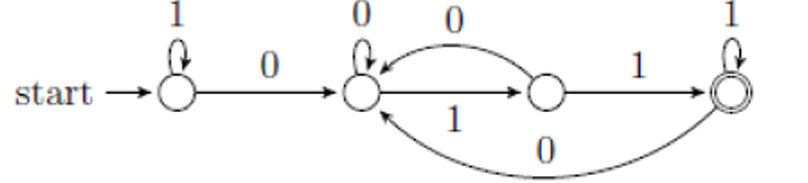
\includegraphics[width=0.3\columnwidth]{figs/q48A.png}
            \label{fig:placeholder}
        \end{figure}
        \item
        \begin{figure}[H]
            \centering
            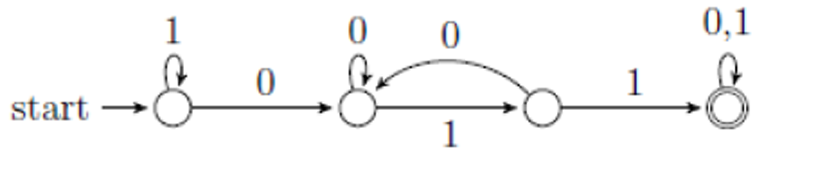
\includegraphics[width=0.3\columnwidth]{figs/q48B.png}
            \label{fig:placeholder}
        \end{figure}
        \item
        \begin{figure}[H]
            \centering
            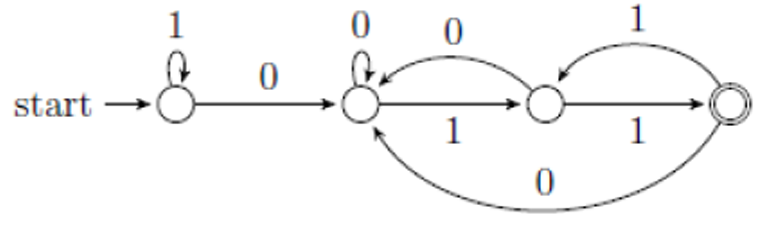
\includegraphics[width=0.3\columnwidth]{figs/q48C.png}
            \label{fig:placeholder}
        \end{figure}
        \item
        \begin{figure}[H]
            \centering
            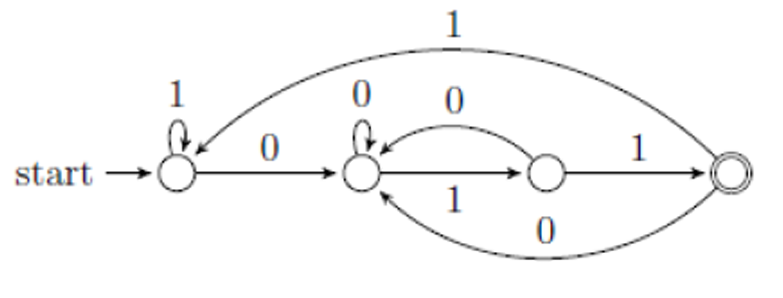
\includegraphics[width=0.3\columnwidth]{figs/q48D.png}
            \label{fig:placeholder}
        \end{figure}
    \end{enumerate}
    \hfill{\brak{\text{GATE CS 2021}}}
    
    \item For a Turing machine M, $\langle M \rangle$ denotes an encoding of M. Consider the following two languages.
    \begin{center}
    $L_1 = \{\langle M \rangle | M \text{ takes more than 2021 steps on all inputs}\}$
    
    $L_2 = \{\langle M \rangle | M \text{ takes more than 2021 steps on some input}\}$ 
    \end{center}
    Which one of the following options is correct?
    \begin{enumerate}
        \item Both $L_1$ and $L_2$ are decidable.
        \item $L_1$ is decidable and $L_2$ is undecidable.
        \item $L_1$ is undecidable and $L_2$ is decidable.
        \item Both $L_1$ and $L_2$ are undecidable.
    \end{enumerate}
    \hfill{\brak{\text{GATE CS 2021}}}
    \item Define $R_n$ to be the maximum amount earned by cutting a rod of length n meters into one or more pieces of integer length and selling them. For $i>0$, let p[i] denote the selling price of a rod whose length is i meters. Consider the array of prices:
    \begin{center}
    $p[1]=1, p[2]=5, p[3]=8, p[4]=9, p[5]=10, p[6]=17, p[7]=18$
    \end{center}    
    Which of the following statements is/are correct about $R_7$?
    \begin{enumerate}
        \item $R_7 = 18$
        \item $R_7 = 19$
        \item $R_7$ is achieved by three different solutions.
        \item $R_7$ cannot be achieved by a solution consisting of three pieces.
    \end{enumerate}
    \hfill{\brak{\text{GATE CS 2021}}}
    
    \item An articulation point in a connected graph is a vertex such that removing the vertex and its incident edges disconnects the graph into two or more connected components.\\Let T be a DFS tree obtained by doing DFS in a connected undirected graph G.\\Which of the following options is/are correct?
    \begin{enumerate}
        \item Root of T can never be an articulation point in G.
        \item Root of T is an articulation point in G if and only if it has 2 or more children.
        \item A leaf of T can be an articulation point in G.
        \item If u is an articulation point in G such that z is an ancestor of u in T and y is a descendent of u in T, then all paths from z to y in G must pass through u.
    \end{enumerate}
    \hfill{\brak{\text{GATE CS 2021}}}
    \item Consider the following Boolean expression.
    \begin{center}
    $F = \brak{X+Y+Z}\brak{\overline{X}+Y}\brak{\overline{Y}+Z}$
    \end{center}
    Which of the following Boolean expressions is/are equivalent to $\overline{F}$ \brak{complement of F}?
    \begin{enumerate}
        \item $\brak{\overline{X}+\overline{Y}+\overline{Z}}\brak{X+\overline{Y}}\brak{Y+\overline{Z}}$
        \item $X\overline{Y}+\overline{Z}$
        \item $\brak{X+\overline{Z}}\brak{\overline{Y}+\overline{Z}}$
        \item $X\overline{Y}+Y\overline{Z}+\overline{X}\overline{Y}\overline{Z}$
    \end{enumerate}
    \hfill{\brak{\text{GATE CS 2021}}}
    \item A relation R is said to be circular if aRb and bRc together imply cRa.\\
    Which of the following options is/are correct?
    
    \begin{enumerate}
        \item If a relation S is reflexive and symmetric, then S is an equivalence relation.
        \item If a relation S is circular and symmetric, then S is an equivalence relation.
        \item If a relation S is reflexive and circular, then S is an equivalence relation.
        \item If a relation S is transitive and circular, then S is an equivalence relation.
    \end{enumerate}
    \hfill{\brak{\text{GATE CS 2021}}}
    
    \item A TCP server application is programmed to listen on port number P on host S. A TCP client is connected to the TCP server over the network.\\Consider that while the TCP connection was active, the server machine S crashed and rebooted. Assume that the client does not use the TCP keepalive timer.\\Which of the following behaviors is/are possible?
    \begin{enumerate}
        \item If the client was waiting to receive a packet, it may wait indefinitely.
        \item The TCP server application on S can listen on P after reboot.
        \item If the client sends a packet after the server reboot, it will receive a RST segment.
        \item If the client sends a packet after the server reboot, it will receive a FIN segment.
    \end{enumerate}
    \hfill{\brak{\text{GATE CS 2021}}}
    
    \item Consider two hosts P and Q connected through a router R. The maximum transfer unit \brak{MTU} value of the link between P and R is 1500 bytes, and between R and Q is 820 bytes.\\A TCP segment of size 1400 bytes was transferred from P to Q through R, with IP identification value as 0x1234. Assume that the IP header size is 20 bytes. Further, the packet is allowed to be fragmented, i.e., Don't Fragment \brak{DF} flag in the IP header is not set by P.\\Which of the following statements is/are correct?
    \begin{enumerate}
        \item Two fragments are created at R and the IP datagram size carrying the second fragment is 620 bytes.
        \item If the second fragment is lost, R will resend the fragment with the IP identification value 0x1234.
        \item If the second fragment is lost, P is required to resend the whole TCP segment.
        \item TCP destination port can be determined by analysing only the second fragment.
    \end{enumerate}
    \hfill{\brak{\text{GATE CS 2021}}}
    
    \item Consider the following pseudocode, where S is a semaphore initialized to 5 in line\#2 and counter is a shared variable initialized to 0 in line\#1. Assume that the increment operation in line\#7 is not atomic.
    
    \begin{verbatim}
1. int counter = 0;
2. Semaphore S = init(5);
3. void parop(void)
4. {
5.     wait(S);
6.     wait(S);
7.     counter++;
8.     signal(S);
9.     signal(S);
10. }
    \end{verbatim}
    
    If five threads execute the function parop concurrently, which of the following program behavior\brak{s} is/are possible?
    \begin{enumerate}
        \item The value of counter is 5 after all the threads successfully complete the execution of parop.
        \item The value of counter is 1 after all the threads successfully complete the execution of parop.
        \item The value of counter is 0 after all the threads successfully complete the execution of parop.
        \item There is a deadlock involving all the threads.
    \end{enumerate}
    \hfill{\brak{\text{GATE CS 2021}}}
    
    \item Consider a dynamic hashing approach for 4-bit integer keys:
    \begin{enumerate}[label=\arabic*.]
        \item There is a main hash table of size 4.
        \item The 2 least significant bits of a key is used to index into the main hash table.
        \item Initially, the main hash table entries are empty.
        \item Thereafter, when more keys are hashed into it, to resolve collisions, the set of all keys corresponding to a main hash table entry is organized as a binary tree that grows on demand.
        \item First, the $3^{rd}$ least significant bit is used to divide the keys into left and right subtrees.
        \item To resolve more collisions, each node of the binary tree is further sub-divided into left and right subtrees based on the $4^{th}$ least significant bit.
        \item A split is done only if it is needed, i.e., only when there is a collision.
    \end{enumerate}
    Consider the following state of the hash table.
    \begin{figure}[h]
        \centering
        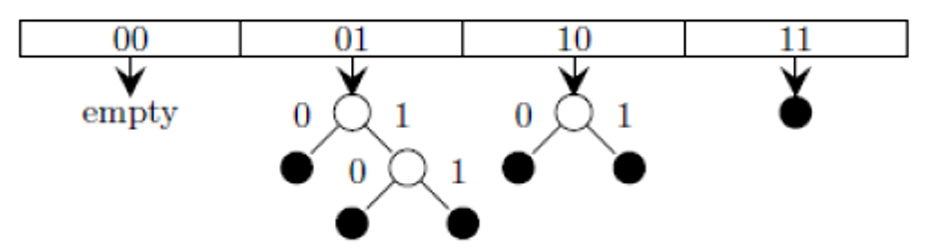
\includegraphics[width=\columnwidth]{figs/q57.png}
        \label{fig:placeholder}
    \end{figure}
    Which of the following sequences of key insertions can cause the above state of the hash table \brak{assume the keys are in decimal notation}?
    
    \begin{enumerate}
        \item $5, 9, 4, 13, 10, 7$
        \item $9, 5, 10, 6, 7, 1$
        \item $10, 9, 6, 7, 5, 13$
        \item $9, 5, 13, 6, 10, 14$
    \end{enumerate}
    \hfill{\brak{\text{GATE CS 2021}}}
    
    \item Consider the following ANSI C function:
    \begin{verbatim}
int SimpleFunction(int Y[], int n, int x)
{
    int total = Y[0], loopIndex;
    for (loopIndex = 1; loopIndex <= n - 1; loopIndex++)
        total = x * total + Y[loopIndex];
    return total;
}
    \end{verbatim}
    Let Z be an array of 10 elements with $Z[i]=1$, for all i such that $0 \le i \le 9$. The value returned by SimpleFunction \brak{Z, 10, 2} is \underline{\hspace{2cm}}.
    
    \hfill{\brak{\text{GATE CS 2021}}}
    
    \item Consider the sliding window flow-control protocol operating between a sender and a receiver over a full-duplex error-free link. Assume the following:
    \begin{itemize}
        \item The time taken for processing the data frame by the receiver is negligible.
        \item The time taken for processing the acknowledgement frame by the sender is negligible.
        \item The sender has infinite number of frames available for transmission.
        \item The size of the data frame is 2,000 bits and the size of the acknowledgement frame is 10 bits.
        \item The link data rate in each direction is 1 Mbps \brak{$=10^6$ bits per second}.
        \item One way propagation delay of the link is 100 milliseconds.
    \end{itemize}
    The minimum value of the sender's window size in terms of the number of frames, \brak{\text{rounded to the nearest integer}} needed to achieve a link utilization of 50\% is \underline{\hspace{2cm}}.
    
    \hfill{\brak{\text{GATE CS 2021}}}
    
    \item Consider the following C code segment:
    
    $a = b + c;$
    
    $e = a + 1;$
    
    $d = b + c;$
    
    $f = d + 1;$
    
    $g = e + f;$
    
    In a compiler, this code segment is represented internally as a directed acyclic graph \brak{DAG}. The number of nodes in the DAG is \underline{\hspace{2cm}}.
    
    \hfill{\brak{\text{GATE CS 2021}}}
    
    \item In a pushdown automaton $P=\brak{Q, \Sigma, \Gamma, \delta, q_0, F}$, a transition of the form,\\ 
    \begin{figure}[H]
        \centering
        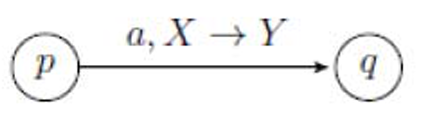
\includegraphics[width=0.3\columnwidth]{figs/q61A.png}
        \label{fig:placeholder}
    \end{figure}
    where p, $q \in Q$, $a \in \Sigma \cup \{\epsilon\}$, and $X, Y \in \Gamma \cup \{\epsilon\}$ represents \\
    \begin{center}
        $\brak{q,Y} \in \delta\brak{p,a,X}$.
    \end{center}
    Consider the following pushdown automaton over the input alphabet $\Sigma = \{a,b\}$ and stack alphabet $\Gamma = \{\#,A\}$.
    \begin{figure}[H]
        \centering
        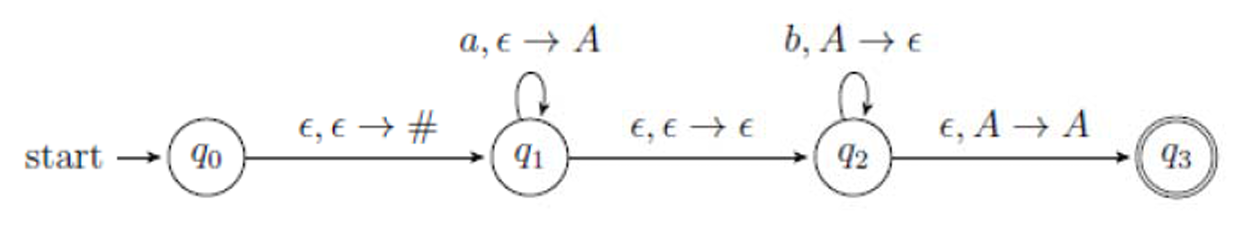
\includegraphics[width=0.5\linewidth]{figs/q61B.png}
        \label{fig:placeholder}
    \end{figure}
    The number of strings of length 100 accepted by the above pushdown automaton is \underline{\hspace{2cm}}.
    
    \hfill{\brak{\text{GATE CS 2021}}}
    
    \item Consider the following matrix.
    \[ \myvec{0 & 1 & 1 & 1 \\ 1 & 0 & 1 & 1 \\ 1 & 1 & 0 & 1 \\ 1 & 1 & 1 & 0} \]
    The largest eigenvalue of the above matrix is \underline{\hspace{2cm}}.
    
    \hfill{\brak{\text{GATE CS 2021}}}
    
    \item A five-stage pipeline has stage delays of 150, 120, 150, 160 and 140 nanoseconds. The registers that are used between the pipeline stages have a delay of 5 nanoseconds each.\\The total time to execute 100 independent instructions on this pipeline, assuming there are no pipeline stalls, is \underline{\hspace{2cm}} nanoseconds.
    \hfill{\brak{\text{GATE CS 2021}}}
    
    \item A sender \brak{S} transmits a signal, which can be one of the two kinds: H and L with probabilities 0.1 and 0.9 respectively, to a receiver \brak{R}.\\In the graph below, the weight of edge \brak{u,v} is the probability of receiving v when u is transmitted, where u, $v \in \{H,L\}$. For example, the probability that the received signal is L given the transmitted signal was H, is 0.7.
    \begin{figure}[H]
        \centering
        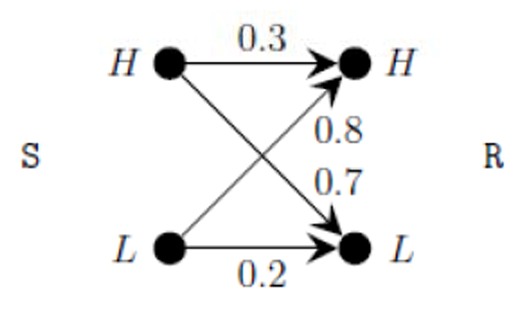
\includegraphics[width=0.5\columnwidth]{figs/q64.png}
        \caption{Caption}
        \label{fig:placeholder}
    \end{figure}
    If the received signal is H, the probability that the transmitted signal was H \brak{rounded to 2 decimal places} is \underline{\hspace{2cm}}.
    
    \hfill{\brak{\text{GATE CS 2021}}}
    
    \item Consider the following instruction sequence where registers R1, R2 and R3 are general purpose and MEMORY[X] denotes the content at the memory location X.
    
    \begin{table}[H]
        \centering
        \begin{tabular}{|l|c|l|}
            \hline
            \textbf{Instruction} & \textbf{Size \brak{bytes}} & \textbf{Semantics} \\
            \hline
            MOV R1, \brak{5000} & 4 & R1 $\leftarrow$ MEMORY[5000] \\
            MOV R2, \brak{R3} & 4 & R2 $\leftarrow$ MEMORY[R3] \\
            ADD R2, R1 & 2 & R2 $\leftarrow$ R1 + R2 \\
            MOV \brak{R3}, R2 & 4 & MEMORY[R3] $\leftarrow$ R2 \\
            INC R3 & 2 & R3 $\leftarrow$ R3 + 1 \\
            DEC R1 & 2 & R1 $\leftarrow$ R1 - 1 \\
            BNZ 1004 & 2 & Branch if not zero to the given absolute address \\
            HALT & 1 & Stop \\
            \hline
        \end{tabular}
        \caption*{}
    \end{table}
    
    Assume that the content of the memory location 5000 is 10, and the content of the register R3 is 3000. The content of each of the memory locations from 3000 to 3010 is 50. The instruction sequence starts from the memory location 1000. All the numbers are in decimal format. Assume that the memory is byte addressable.\\After the execution of the program, the content of memory location 3010 is \underline{\hspace{2cm}}.
    \hfill{\brak{\text{GATE CS 2021}}}

\end{enumerate}
\end{document}
